Zur Berechnung der Magnetisierung wird die Korrelation zweier beliebig weit entfernter Spins benötigt. Da das Gitter isotrop und homogen ist, reicht es aus sich auf die Berechnung der horizontalen Spin-Spin-Korrelation $\corr{\sigma_{0,0}\,\sigma_{m,0}}$ zu beschränken.
Diese soll nun in diesem Abschnitt berechnet werden.

\subsection{Spin-Spin-Korrelationen ausgedrückt als Graßmann-Korrelationen}

Ausgangspunkt ist Gleichung \eqref{eq: Defekte Zustanssumme}, mithilfe der sich die Spin-Spin-Korrelation $\corr{\sigma_i \sigma_j}$ als Quotient zweier Zustandssummen schreiben lässt. Die Zustandssumme im Zähler ist dabei die eines defekten Gitters. Die Gitterdefekte, sowie die zugehörigen Gitterpunkte, zusammengefasst in $L_D$, liegen in diesem Fall alle auf einer Geraden parallel zur x-Achse.
\begin{equation}
L_D = \{ x \;\;|\;\;  \exists\, l \in \{0, \dots, m-1\} : x = (l, 0)\}
\end{equation}

\noindent Da sich die Vorfaktoren der Zustandssummen kürzen, kann dieser Ausdruck mithilfe von \eqref{eq: Zustandssumme-GV-Darstellung} als Quotient zweier Berezin-Integrale geschrieben werden. 
\begin{equation} \label{eq: corr_as_Berezion_int}
\corr{\sigma_{x,y} \sigma_{x+m,y}}  = \frac{t^m \, \tilde{Z}_D}{\tilde{Z}} \approx \frac{t^m \, \Sp{\mathrm{e}^{A_D}}}{\Sp{\mathrm{e}^A}}
\end{equation}

\noindent Die Gleichheit gilt wieder nur asymptotisch im Thermodynamischen Limes. $A$ ist dabei die Graßmann-Wirkung des isotropen 2d Ising-Gitters und $A_D$ die des defekten Gitters. Diese stehen über \eqref{eq: G_Wikrung_Defekt} miteinander in Zusammenhang.
\begin{equation} \label{eq: G_Wikrung_Defekt}
A_D = A - \sum_{x \in \Lambda_D} t\, h_{\bm{x}}^x\, h_{\bm{x} + \bm{e}_x}^o + \sum_{x_k \in \Lambda_D} t^{-1}\, h_{\bm{x}_k}^x\, h_{\bm{x}_k + \bm{e}_x}^o
\end{equation}

\noindent Unter Verwendung der Tatsache dass Paare von Graßmann Variablen kommutieren und \eqref{eq: G_Wikrung_Defekt} lässt sich $\mathrm{e}^{A_D}$ dann gemäß 
\begin{align}
e^{A_D} 
    & = e^{A} \prod_{x \in \Lambda_D} \exp{(t^{-1} - t)\, h_{\bm{x}}^x\, h_{\bm{x} + \bm{e}_x}^o} \nonumber \\
    & = e^{A} \prod_{x \in \Lambda_D} 1 + (t^{-1} - t)\, h_{\bm{x}}^x\, h_{\bm{x} + \bm{e}_x}^o \nonumber \\
    & = e^{A} \prod_{l = 0}^{m-1} 1 + (t^{-1} - t)\, h_{l,0}^x\, h_{l+1,0}^o \label{eq: coor_fun}
\end{align}
umschreiben. Setzt man \eqref{eq: coor_fun} in \eqref{eq: corr_as_Berezion_int} ein, erkennt man dass sich die Spin-Spin-Korrelation als Korrelation einer Graßmann-Funktion schreiben lässt.  
\begin{equation} \nonumber
\corr{\sigma_{x,y} \sigma_{x+m,y}} 
    =\frac{t^m \, \Sp{\mathrm{e}^{A_D}}}{\Sp{\mathrm{e}^A}} 
    =  t^m \, \corr{\prod_{l = 0}^{m-1} 1 + (t^{-1} - t)\, h_{l,0}^x\, h_{l+1,0}^o} 
\end{equation}

\noindent Durch Ausmultiplizieren des Produktes und unter Verwendung der Linearität der Korrelation lässt sich die Spin-Spin-Korrelation als Summe von Graßmann-Korrelationen beschreiben. 
\begin{align}
\prod_{l = 0}^{m-1} 1 + (t^{-1} - t)\, h_{l,0}^x\, h_{l+1,0}^o
= 1 + \sum_{k = 1}^{m} (t^{-1}-t)^k \sum_{l_1 < \dots < l_k} h_{l_1,0}^x\, h_{l_1+1,0}^o \cdots h_{l_k,0}^x\, h_{l_k+1,0}^o
\end{align}

\begin{grayframe}[frametitle = {Spin-Spin-Korrelation als Summe von Graßmann-Korrelationen}]
\begin{equation} \label{eq: Spin-Spin-Corr as Sum of GV corr}
    \corr{\sigma_{0,0} \sigma_{m,0}} = t^m  + \sum_{k = 1}^{m} t^{m-k} \, (1-t^2)^{k} \sum_{l_1 < \dots < l_k}  \corr{h_{l_1,0}^x\, h_{l_1+1,0}^o \cdots h_{l_k,0}^x\, h_{l_k+1,0}^o}
\end{equation}
\end{grayframe}

\subsection{Berechnung von Graßmann-Paar-Korrelationen}
Um \eqref{eq: Calculate_GV_Corr} zur Berechung der Korrelationen nutzen zu können, muss die darstellende Matrix der Graßmanm-Dichte ${\mathrm{e}^A}$ bekannt sein. Da die darstellende Matrix für den Satz fouriertransformierter Graßmann-Variablen eine einfache Gestalt hat, bietet es sich an die Berechnung für diese durchzuführen und dann über die Fouriertransformation die ursprüngliche Korrelation zu berechnen. 

\subsubsection{Fouriertransformation der Korrelationen}
Aufgrund der Homogenität und der periodischen Randbedingungen sind die Graßmann-Korrelationen translationsinvariant. Daher ergibt sich 
\begin{equation} \label{eq: gv_multi_translation}
\corr{\eta_{\bm{x}_l}^{\nu}\, \eta_{\bm{x}_{l'}}^{\nu'} } = \frac{1}{N} \sum_{\bm{x} \in \Lambda} \corr{\eta_{\bm{x}_l + \bm{x}}^{\nu} \,\eta_{\bm{x}_{l'} + \bm{x}}^{\nu'} }
\end{equation}
Dabei indiziert $\nu$, wie schon in Abschnitt \ref{sec: Fouriertransformation der Graßmann-Wirkung}, wieder eine der vier Familien von Graßmann-Variablen auf dem Gitter. 
\noindent Durch Einsetzen der Definiton \eqref{eq: Fourer2D invers} für die Fouriertransformation in die Graßmann-Paar-Korrelation, erhält man die folgende Darstellung in den fouriertransformierten Variablen.
\begin{align} \label{eq: ft_gv_pair_corr}
\frac{1}{N} \sum_{\bm{x} \in \Lambda} \corr{\eta_{\bm{x}_l + \bm{x}}^{\nu} \,\eta_{\bm{x}_{l'} + \bm{x}}^{\nu'} }
& = \frac{1}{N} \sum_{\bm{x} \in \Lambda} \; \corr{\frac{1}{\sqrt{N}} \sum_{\bm{k} \in \bar{\Lambda}} \hat{\eta}_{\bm{k}}^{\nu}\; \mathrm{e}^{-i \bm{k} \cdot (\bm{x}_l + \bm{x})} \frac{1}{\sqrt{N}} \sum_{\bm{k'} \in \bar{\Lambda}} \hat{\eta}_{\bm{k'}}^{\nu'}\; \mathrm{e}^{-i  \bm{k'} \cdot (\bm{x}_{l'}+\bm{x})}} \nonumber \\
&  = \frac{1}{N} \sum_{\bm{k} \in \bar{\Lambda}} \sum_{\bm{k'} \in \bar{\Lambda}} \mathrm{e}^{-i  (\bm{k} \cdot \bm{x}_l + \bm{k'} \cdot \bm{x}_{l'})} \, \corr{\hat{\eta}_{\bm{k}}^{\nu}\, \hat{\eta}_{\bm{k'}}^{\nu'}} \, \frac{1}{N} \sum_{\bm{x} \in \Lambda} \mathrm{e}^{-i (\bm{k} + \bm{k'})\cdot \bm{x} } \nonumber \\ 
&  = \frac{1}{N} \sum_{\bm{k} \in \bar{\Lambda}} \sum_{\bm{k'} \in \bar{\Lambda}} \mathrm{e}^{-i  (\bm{k} \cdot \bm{x}_l + \bm{k'} \cdot \bm{x}_{l'})} \, \corr{\hat{\eta}_{\bm{k}}^{\nu} \, \hat{\eta}_{\bm{k'}}^{\nu'}} \; \delta(\bm{k} + \bm{k'}) \nonumber \\
& = \frac{1}{N} \sum_{\bm{k} \in \bar{\Lambda}}  \mathrm{e}^{-i  \bm{k} \cdot (\bm{x}_l - \bm{x}_{l'})} \,\corr{\hat{\eta}_{\bm{k}}^{\nu}\, \hat{\eta}_{-\bm{k}}^{\nu'}} \nonumber
\end{align}

\noindent Die Korrelationen die zur Berechnung von \eqref{eq: Spin-Spin-Corr as Sum of GV corr} benötigt werden, liegen alle auf einer Linie parallel zur x-Achse. Daher ergibt sich letztlich die folgenden Darstellungen für die Fouriertransformation der horizontalen Korrelationen.

\begin{grayframe}[frametitle = {Fouriertransformierte horizontale Graßmann-Korrelationen}]
\begin{equation} \label{eq: horz_gv_pair_corr}
\corr{\eta^{\nu}_{(l,0)}\, \eta^{\nu'}_{(l', 0)} } = \frac{1}{N} \sum_{\bm{k} \in \bar{\Lambda}}  \mathrm{e}^{-i\,(l- l') \,k_1} \,\corr{\hat{\eta}_{\bm{k}}^{\nu}\, \hat{\eta}_{-\bm{k}}^{\nu'}}
\end{equation} 
\end{grayframe}

\subsubsection{Korrelationen im K-Raum}

Zur Berechnung der Paar-Korrelationen im K-Raum nutzt man die Formel \eqref{eq: Calculate_GV_Corr} zur Berechnung der Korrelation über die Inverse der darstellende Matrix der Graßmann-Dichte. Danach ergibt sich 
\begin{equation} 
    \corr{\hat{\eta}_{\bm{k}}^{\nu}\, \hat{\eta}_{-\bm{k}}^{\nu'}}_{\Lambda_N} = \frac{\Sp{\mathrm{e}^{\hat{A}}\hat{\eta}_{\bm{k}}^{\nu}\, \hat{\eta}_{-\bm{k}}^{\nu'}}}{\Sp{\mathrm{e}^{\hat{A}}}} = pf(-(2\bm{\hat{A}}^{-1})^{II}) 
\end{equation} 
als zu berechnender Ausdruck. $I = \{i_{1}, i_{2} \} $ ist dabei die Indexmenge der relevanten Zeilen und Spalten. $i_{1}$ ist der zu $ \hat{\eta}_{\bm{k}}^{\nu} $ gehörige  und $i_{2}$ der zu $\hat{\eta}_{-\bm{k}}^{\nu'}$ gehörige Index. Aufgrund der gewählten Numerierung der Gitterpunkte, gilt $i_{1} < i_2$. Die Matrix $(\bm{\hat{A}}^{-1})^{II}$ erhält man durch Streichen aller Zeilen und Spalten von $\bm{A}$ , deren Indices nicht in $I$ liegen. In diesem Fall handelt es sich um eine $2\times2$ Matrix,  deren Pfaffsche Determinante
\begin{equation}
 \pf{(-2\bm{\hat{A}})^{-1})^{II}} = \pf{\begin{array}{cc} 
        0 & -\left((2\hat{A})^{-1}\right)_{i_1,i_2}     \\
        -\left((2\hat{A})^{-1}\right)_{i_2,i_1} & 0
    \end{array}} 
    = -\left((2\bm{\hat{A}})^{-1}\right)_{i_1,i_2}
\end{equation}
vollständig durch $(2\bm{\hat{A}}^{-1})_{i_1,i_2}$ bestimmt ist. Bei der Berechnung dieses Matrixelements kommt einem die Blockmatrix-Form von $\bm{\hat{A}}$ zugute, welche bei der Inversion ebenfalls erhalten bleibt. Unter Beachtung der Tatsache dass $\bm{\hat{A}}_{-\bm{k}_i} = \bm{\hat{A}}_{\bm{k}_{i+2M(M+1)}}$  gilt, überprüft man leicht durch nachrechnen, dass die Inverse der Matrix $\bm{\hat{A}}$ die folgende Form haben muss. 
\begin{equation}
(2\bm{\hat{A}})^{-1} = 
\left(\begin{array}{c|ccc|ccc}  
\bm{\hat{A}}_{\bm{k}_0}^{-1}  & \bm{0}   & \cdots    & \bm{0} & \bm{0} & \cdots  & \bm{0} \\ \hline
\bm{0}  & \bm{0}       & \cdots   & \bm{0}    & \bm{\hat{A}}_{-\bm{k}_{1}}^{-1} & \cdots  & \bm{0} \\
\vdots  &\vdots        & \ddots   & \vdots    & \vdots                  & \ddots  & \vdots \\
\bm{0}  & \bm{0}       & \cdots   & \bm{0} & \bm{0} & \cdots  & \bm{\hat{A}}_{-\bm{k}_{2M(M+1)}}^{-1}  \\ \hline
\bm{0}  & \bm{\hat{A}}_{\bm{k}_1}^{-1} & \cdots  & \bm{0} & \bm{0} & \cdots  & \bm{0} \\
\vdots  &\vdots        & \ddots   & \vdots    & \vdots                  & \ddots  & \vdots \\
\bm{0}  & \bm{0}       & \cdots   & \bm{\hat{A}}_{\bm{k}_{2M(M+1)}}^{-1}& \bm{0} & \cdots  & \bm{0} 
\end{array} \right) 
\end{equation}

\noindent Das Matrixelement das zu $I$ gehört, liegt dann in der Matrix $\bm{\hat{A}}_{-\bm{k}}^{-1}$. Spalte und Zeile in  $\bm{\hat{A}}_{-\bm{k}}^{-1}$ werden dann von der Familie der zugehörigen Graßmann-Variablen bestimmt. Einzelne Matrixelemnte der $4\times4$ Matrix lassen sich mithilfe der Cramer'schen Regel bestimmen. Die Matrizen $\bm{\hat{A}_{\bm{k}}}$ wurde in Abschnitt \ref{sec: Fouriertransformation der Graßmann-Wirkung} aufgestellt. Ihre Struktur ist hier noch einmal aufgeschlüsselt.
\begin{equation} \label{eq: struct A_k}
\renewcommand{\arraystretch}{1.5}
    \bm{\hat{A}}_{\bm{k}} : \;\;\;\; \begin{array}{c|c:c:c:c} 
                           & \hat{h}_{-\bm{k}}^o & \hat{h}_{-\bm{k}}^x & \hat{v}_{-\bm{k}}^o & \hat{h}_{-\bm{k}}^x  \\ \hline
        \hat{h}_{\bm{k}}^o & 0                   & -\xi(-k_1)            &  1                  & 1                   \\ \hdashline
        \hat{h}_{\bm{k}}^x & \xi(k_1)          & 0                   &  -1                  &  1                   \\ \hdashline
        \hat{v}_{\bm{k}}^o &-1                   & 1                  &  0                  & -\xi(-k_2)             \\ \hdashline
        \hat{v}_{\bm{k}}^x & -1                   & -1                  &\xi(k_2)           &  0                   \\ 
    \end{array}
\end{equation}
Für die Berechnung der Inversen mit der Cramer'schen Regel wird die Determinante 
\begin{equation} \label{eq: expl det(A_K) xi} 
\det{\bm{\hat{A}}_{\bm{k}}} = \xi(k_1)\xi(-k_1)\xi(k_2)\xi(-k_2) -(\xi(k_1)+\xi(-k_1))(\xi(k_2)+\xi(-k_2)) + 4 
%det(\bm{\hat{A}}_{\bm{k}}) = (1+t^2)^2 - 2t(1-t^2)\,(\cos(k_1) + \cos(k_2))
\end{equation}
der Matrix $\bm{\hat{A}}_{\bm{k}}$ benötigt. Mithilfe der Zwischenergebnisse
\begin{align} \nonumber
\xi(k)+\xi(-k) &= 2(1 + t\,\cos(k)) \nonumber \\
\xi(k)\xi(-k) &= 1 + 2t\,\cos(k) + t^2 \nonumber
\end{align} kann dieses Ergebnis weiter aufgelöst werden. Nach einigen weiteren algebraischen Umformung erhält man dann
\begin{equation} \label{eq: expl. det(A_k)}
\det{\bm{\hat{A}}_{\bm{k}}}
    = (1+t^2)^2 - 2t(1-t^2)\,(\cos(k_1) + \cos(k_2))
\end{equation}
für die Determinante.
Nun müssen die einzelnen Fälle explizit unterschieden werden. Für $\corr{\hat{h}_{\bm{k}}^x\, \hat{h}_{-\bm{k}}^o} $ ergibt sich 
\begin{equation} \nonumber
((2\bm{\hat{A}})^{-1})_{i_1,i_2} = ((\bm{\hat{A}}_{-\bm{k}})^{-1})_{2,1}
\end{equation}
für das zu bestimmende Matrixelement. Mit der Cramer'schen Regel ergibt sich dann
\begin{align}
\det{\bm{\hat{A}}_{-\bm{k}}} ((\bm{\hat{A}}_{-\bm{k}})^{-1})_{2,1}  &= 
\left\vert \begin{array}{cccc} 
 0          & 1    &  1             & 1                   \\
 \xi(-k_1)  & 0    &  -1            &  1                   \\ 
-1          & 0    &  0             & -\xi(k_2)             \\ 
-1          & 0    &  \xi(-k_2)      &  0                   \\ 
    \end{array}
\right\vert \nonumber\\
& = \xi(k_2) + \xi(-k_2) - \xi(-k_1)\xi(k_2)\xi(-k_2)  \nonumber   
\end{align}
Unter Ausnutzung der Symetrie $\det{\bm{\hat{A}}_{-\bm{k}}} = \det{\bm{\hat{A}}_{\bm{k}}} $ folgt dann
\begin{align} \nonumber
\pf{-(2\bm{A}^{-1})^{II}} = \frac{\xi(-k_1)\xi(k_2)\xi(-k_2) -\xi(k_2) - \xi(-k_2) }{ \det{\bm{\hat{A}}_{\bm{k}}}}  
\end{align}
und somit 
\begin{grayframe}[frametitle = {Horizontale Graßmann-Paar-Korrelation im K-Raum}]
\begin{equation} \label{eq: expl grassmann_pair_corr}
\corr{\hat{h}_{\bm{k}}^x\, \hat{h}_{-\bm{k}}^o}_{\Lambda_N} = \frac{\xi(-k_1)\xi(k_2)\xi(-k_2) -\xi(k_2) - \xi(-k_2)}{(1+t^2)^2 - 2t(1-t^2)\,(\cos(k_1) + \cos(k_2))}
\end{equation}
\end{grayframe}
\noindent Für die anderen zwei Korrelationen verfährt man analog. Für $\corr{\hat{h}_{\bm{k}}^o\, \hat{h}_{-\bm{k}}^o} $ muss man das Matrixelement $-((\bm{\hat{A}}_{-\bm{k}})^{-1})_{1,1}$ und für  $\corr{\hat{h}_{\bm{k}}^x\, \hat{h}_{-\bm{k}}^x} $ das Matrixelement $-((\bm{\hat{A}}_{-\bm{k}})^{-1})_{2,2}$ berechnen. Man erhält dann, nach dem Rückeinsetzen für $\xi(.)$, das folgende Ergebnis.
\begin{grayframe}
\begin{equation} \label{eq: expl grassmann_pair_corr 0}
\corr{\hat{h}_{\bm{k}}^o\, \hat{h}_{-\bm{k}}^o}_{\Lambda_N} \propto \corr{\hat{h}_{\bm{k}}^x\, \hat{h}_{-\bm{k}}^x}_{\Lambda_N} \propto \frac{2i\,\sin(k_2)}{(1+t^2)^2 - 2t(1-t^2)\,(\cos(k_1) + \cos(k_2))} 
%\corr{\hat{h}_{\bm{k}}^x\, \hat{h}_{-\bm{k}}^x} = \corr{\hat{h}_{\bm{k}}^o\, \hat{h}_{-\bm{k}}^o} \propto \frac{\xi(k_2) -\xi(-k_2)}{(1+t^2)^2 - 2t(1-t^2)\,(\cos(k_1) + \cos(k_2))} 
\end{equation}
\end{grayframe}



\subsubsection{Übergang in den Thermodynamischen Limes}
Wenn man an die Definition \eqref{def: Brillouin-Zone} der Vektoren $\bm{k}$ zurückdenkt, so erkennt man mit der Korrespondenz 

\begin{equation} \label{eq: Korrespondez Integral_Summe Tlim 1}
\bm{k} = (k_1, k_2)  =  (\frac{2\pi q_1}{2M+1}, \frac{2\pi q_2}{2M+1}) 
\end{equation}
dass

\begin{equation} \label{eq: Korrespondez Integral_Summe Tlim 2}
\frac{1}{N} = \frac{1}{(2M+1)^2} = \Delta q_1 \Delta q_2 = \frac{\Delta k_1}{2\pi}\frac{\Delta k_2}{2\pi} 
\end{equation}
gilt. Damit kann der Ausdruck in \eqref{eq: horz_gv_pair_corr} dann als Riemann-Summe identifiziert werden. Diese konvergiert dann im Thermodymischen Limes gegen ein Integral über die gesamte erste Brillouin-Zone. 
\begin{equation} \nonumber
\sum_{\bm{k} \in \bar{\Lambda}}  \mathrm{e}^{-i\,(l-l') \,k_1} \,\corr{\hat{\eta}_{\bm{k}}^{\nu}\, \hat{\eta}_{-\bm{k}}^{\nu'}}_{\Lambda_N} \frac{\Delta k_1}{2\pi}\frac{\Delta k_2}{2\pi} \;\xrightarrow[\substack{\Delta k_1 \rightarrow 0 \\ \Delta k_2 \rightarrow 0 }]{}\; \frac{1}{(2\pi)^2}\int_{-\pi}^{\pi} \int_{-\pi}^{\pi} \d k_1 \d k_2 \,\,\mathrm{e}^{-i\, (l-l') \,k_1} \corr{\hat{\eta}_{\bm{k}}^{\nu}\, \hat{\eta}_{-\bm{k}}^{\nu'}}_{\Lambda_N} 
\end{equation} 

\noindent Mit den Substitutionen 
\begin{align}
\kappa = 2t(1-t^2) \label{subs: kappa}\\
\gamma = (1+t^2)^2 \label{subs: gamma}\\
\Omega(k_1) = \gamma - \kappa\, \cos(k_1) \label{subs: omega} 
\end{align}
\noindent folgt für das Integral der Korrelation $\corr{h^{x}_{(l,0)}\, h^{x}_{(l', 0)} }$
\begin{equation} \nonumber
\frac{1}{(2\pi)^2}\int_{-\pi}^{\pi} \int_{-\pi}^{\pi} \d k_1 \d k_2 \,\,\mathrm{e}^{-i\,(l-l') \,k_1} \corr{\hat{h}_{\bm{k}}^{x}\, \hat{h}_{-\bm{k}}^{x}}_{\Lambda_N} \propto  \int_{-\pi}^{\pi} \d k_2 \frac{\sin(k_2)}{\Omega(k_1) - \kappa \cos(k_2)} = 0 ,
\end{equation}
da der Integrand eine ungerade Funktion in $k_2$ ist. Die Korrelation $\corr{h^{o}_{(l,0)}\, h^{o}_{(l', 0)} } $ verschwindet dann ebenfalls im Thermodynamischen Limes. Für die verbliebene Korrelation setzt man schließlich den Ausdruck \eqref{eq: expl grassmann_pair_corr} für die Graßmann-Korrelation im Integral ein. Zusammengefasst erhält man dann das folgende Ergebnis.

\begin{grayframe}[frametitle = {Horizontale Graßmann-Korrelationen für das unendliche 2d Ising-Gitter}]
\begin{equation} 
\corr{h^{x}_{(l,0)}\, h^{o}_{(l', 0)} } = \frac{1}{(2\pi)^2}\int_{-\pi}^{\pi} \int_{-\pi}^{\pi} \d k_1 \d k_2 \,\,\mathrm{e}^{-i\, (l-l') \,k_1} \frac{F_{\xi}(k_1,k_2)}{\Delta(k_1, k_2)}  \label{eq: corr Integral}
\end{equation}
\begin{align}
F_{\xi}(k_1,k_2) &= \xi(-k_1)\xi(k_2)\xi(-k_2) -\xi(k_2) - \xi(-k_2) \\
\Delta(k_1, k_2) &= (1+t^2)^2 - 2t(1-t^2)\,(\cos(k_1) + \cos(k_2))
\end{align}
\begin{equation} \label{eq: hxhx and hoho is null}
\corr{h^{x}_{(l,0)}\, h^{x}_{(l', 0)} } = 
\corr{h^{o}_{(l,0)}\, h^{o}_{(l', 0)} } = 0
\end{equation}
\end{grayframe}

\subsection{Berechnung der Spin-Spin-Korrelationen}
Ausgangspunkt ist Gleichung \eqref{eq: Spin-Spin-Corr as Sum of GV corr} nach der sich
\begin{equation} \nonumber
    \corr{\sigma_{0,0} \sigma_{m,0}} = t^m  + \sum_{k = 1}^{m} t^{m-k} \, (1-t^2)^{k} \sum_{l_1 < \dots < l_k}  \corr{h_{l_1,0}^x\, h_{l_1+1,0}^o \cdots h_{l_k,0}^x\, h_{l_k+1,0}^o}
\end{equation} für den Zusammenhang zwischen Spin-Spin-Korrelation und Graßmann-Korrelationen ergibt. Durch Auswerten der Graßmann-Korrelationen als Paar-Korrelationen wird nun gezeigt, dass sich die Spin-Spin-Korrelation als Determinante einer geeigneten Matrix $\bm{C}$ schreiben lässt, deren Einträge durch die bereits berechneten Graßmann-Paar-Korrelationen bestimmt ist. \\
\newpage
\noindent Es sei nun $I = \{l_1,\dots,l_k\}$ die Indexmenge der Korrelationen $\corr{h_{l_1,0}^x\, h_{l_1+1,0}^o \cdots h_{l_k,0}^x\, h_{l_k+1,0}^o}$.
Mit \eqref{eq: calc monom corr with pair corr matrix} erhält man dann
\begin{equation}
 \corr{h_{l_1,0}^x\, h_{l_1+1,0}^o \cdots h_{l_k,0}^x\, h_{l_k+1,0}^o} = \corr{\prod_{l \in I} h_{l,0}^x\, h_{l+1,0}^o} = pf(\bm{M}_I ) \\
\end{equation}
für die Korrelationen. Die Matrix $\bm{M}_I$ ist gemäß
\begin{equation}
\bm{M}_I 
    = \left(\begin{array}{cccccc} 
      \corr{h_{l_1,0}^x\, h_{l_1,0}^x}  &  \corr{h_{l_1,0}^x\, h_{l_1+1,0}^o} & \corr{h_{l_1,0}^x\, h_{l_2+1,0}^x} & \cdots & \corr{h_{l_1,0}^x\, h_{l_k+1,0}^o} \\
      \corr{h_{l_1+1,0}^o\, h_{l_1,0}^x}  &  \corr{h_{l_1+1,0}^o\, h_{l_1+1,0}^o} & \corr{h_{l_1+1,0}^o\, h_{l_2+1,0}^x} & \cdots & \corr{h_{l_1+1,0}^o\, h_{l_k+1,0}^o} \\
      \corr{h_{l_2,0}^x\, h_{l_1,0}^x}  &  \corr{h_{l_2,0}^x\, h_{l_1+1,0}^o} & \corr{h_{l_2,0}^x\, h_{l_2+1,0}^x} & \cdots & \corr{h_{l_2,0}^x\, h_{l_k+1,0}^o} \\ 
      \vdots & \vdots & \vdots & \ddots & \vdots \\
      \corr{h_{l_k+1,0}^o\, h_{l_1,0}^x}  &  \corr{h_{l_k+1,0}^o\, h_{l_1+1,0}^o} & \corr{h_{l_k+1,0}^o\, h_{l_2+1,0}^x} & \cdots & \corr{h_{l_k+1,0}^o\, h_{l_k+1,0}^o} \\
      \end{array}\right)
\end{equation}
 definiert. Die Hälfte der Einträge in $\bm{M}_I$ sind jedoch Null, denn nach dem früheren Ergebnis \eqref{eq: hxhx and hoho is null} gilt $\corr{h_{l,0}^x,h_{l',0}^x} = \corr{h_{l,0}^o,h_{l',0}^o} = 0$. Mithilfe der Matrix $\tilde{C}_{l,l'} = \corr{h_{l-1,0}^x h_{l',0}^o}$ lässt sich die Gestalt der Matrix $\bm{M}_I $ dann erheblich vereinfachen.

\begin{equation}
\bm{M}_I 
    = \left(\begin{array}{ccccccc} 
      0 & \tilde{C}_{l_1,l_1} & 0 &\tilde{C}_{l_1,l_2} & \cdots & \tilde{C}_{l_1,l_k} \\
      - \tilde{C}_{l_1,l_1} & 0 & -\tilde{C}_{l_2,l_1} & 0 & \cdots & 0 \\
      0 & \tilde{C}_{l_2,l_1} & 0 & \tilde{C}_{l_2,l_2}  & \cdots & \tilde{C}_{l_2,l_k} \\
      \vdots & \vdots & \vdots & \vdots  & \ddots & \vdots \\
      - \tilde{C}_{l_1,l_k} & 0 & -\tilde{C}_{l_2,l_k}  & 0 & \cdots & 0 \\
      \end{array}\right)
\end{equation}

\noindent Durch eine entsprechende Permutation $P$ der Zeilen und Spalten lassen sich weitere Vereinfachungen vornehmen. 
\begin{equation}
    \bm{P}^T\bm{M}_I \bm{P} 
    = \left(\begin{array}{ccccccc} 
      0 & \cdots & 0 & \tilde{C}_{l_1,l_1} & \cdots & \tilde{C}_{l_1,l_k} \\
      \vdots & \ddots & \vdots & \vdots  & \ddots & \vdots \\
      0 & \cdots & 0 & \tilde{C}_{l_k,l_1} & \cdots & \tilde{C}_{l_k,l_k} \\
      -\tilde{C}_{l_1,l_1} & \cdots & -\tilde{C}_{l_k,l_1} & 0 & \cdots & 0   \\
      \vdots & \ddots & \vdots & \vdots  & \ddots & \vdots \\
      -\tilde{C}_{l_1,l_k} & \cdots & -\tilde{C}_{l_k,l_k} & 0 & \cdots & 0   \\
    \end{array}\right) 
    =: \left(\begin{array}{cc}
      \bm{0} & \bm{\tilde{C}}^{II} \\
      -(\bm{\tilde{C}}^{II})^T & \bm{0}
    \end{array}\right) 
\end{equation}

\noindent Für das Vorzeichen der Permutation $P$ gilt $\sign{P} = \det{\bm{P}} = (-1)^{k(k-1)/2}$, wie in Abb. \ref{Abb: Permutation für M_I} veranschaulicht. Mithilfe der Anti-Diagnoanlblock-Formel \eqref{eq:pfaff 6} für Pfaffsche Determinanten erhält man dann, dass sich die Korrelationen als Hauptminoren der Matrix $\bm{\tilde{C}}$ schreiben lassen.  
\begin{alignat}{2} 
\corr{\prod_{l \in I} h_{l,0}^x\, h_{l+1,0}^o} 
&= \pf{\bm{P} \left(\begin{array}{cc}
      \bm{0} & \bm{\tilde{C}}^{II} \\
      -(\bm{\tilde{C}}^{II})^T & 0
    \end{array}\right)  \bm{P}^T} && \nonumber\\
& = ((-1)^{k(k-1)/2})^2 \; \det{\bm{\tilde{C}}^{II}} &&= \det{\bm{\tilde{C}}^{II}} \label{eq: corr is minor of C}
\end{alignat}


\noindent Mithilfe eines Satzes aus der Linearen Algebra lässt sich damit die Spin-Spin-Korrelation, in der Form \eqref{eq: Spin-Spin-Corr as Sum of GV corr},  auf das charakteristische Polynom der Matrix $\bm{\tilde{C}}$ zurückführen (Beweis des Satzes in Appendix \ref{appendix: Satz über Koeffizienten des Charakteristischen Polynoms}).

\begin{grayframe}[frametitle = {Satz über die Koeffizienten des charackteristischen Polynoms}]

Sei $\bm{A}\in \mathbb{C}^{m\times m}$ eine beliebige komplexe Matrix. Die Koeffizienten des charackteristischen Polynoms lassen sich gemäß \eqref{satz: coeffs of char-polynom E_k} mithilfe der Hauptminoren $\det{\bm{A}^{II}}$ der Matrix $\bm{A}$ ausdrücken. $\bm{A}^{II} \in  \mathbb{C}^{k\times k}$ erhält man indem man die Zeilen und Spalten mit Indices, die nicht in $I\subseteq \{1,\dots,n\}$ liegen, in $\bm{A}$ streicht. 
\begin{equation} \label{satz: coeffs of char-polynom}
p_{\bm{A}}(\lambda) = det(A - \lambda) = (-1)^m \;\lambda^m + \sum_{k = 0}^{m-1} (-1)^k \;E_{m-k} \;\lambda^k
\end{equation}
\begin{equation} \label{satz: coeffs of char-polynom E_k}
E_k = \sum_{{I} \subseteq \{1,\dots,m\} }^{\#^{II} = k} \det{\bm{A}^{II}}
\end{equation}
\end{grayframe}

\noindent Mihilfe der Identifikation von \eqref{satz: coeffs of char-polynom E_k} und \eqref{eq: corr is minor of C} kann man Zusammenhang 

\begin{equation}
\sum_{l_1 < \dots < l_k}  \corr{h_{l_1,0}^x\, h_{l_1+1,0}^o \cdots h_{l_k,0}^x\, h_{l_k+1,0}^o} = \sum_{{I} \subseteq \{1,\dots,m\} }^{\#I = k} \det{\bm{\tilde{C}}^{II}} = E_{k}
\end{equation}
erkennen. Aus Vergleich von \eqref{satz: coeffs of char-polynom} und \eqref{eq: Spin-Spin-Corr as Sum of GV corr} ergibt sich dann schließlich die Spin-Spin-Korrelation als das charakteristische Polynom der Matrix $(1-t^2)\bm{\tilde{C}}$ ausgewertet an der Stelle $\lambda = -t$.
\begin{align}
 \corr{\sigma_{0,0}\, \sigma_{m,0}} 
 &= t^m  + \sum_{k = 1}^{m} t^{m-k} \, (1-t^2)^{k} \sum_{I \subseteq \{1,\dots,m\} }^{\#I = k} \det{\bm{\tilde{C}}^{II}} \nonumber \\
 &= (-1)^m\,(-t)^m  + \sum_{k' = 0}^{m-1} t^{k'} \, (1-t^2)^{m-k'} \sum_{I \subseteq \{1,\dots,m\} }^{\#I = m-k'} \det{\bm{\tilde{C}}^{II}} \nonumber\\
 &= (-1)^m\,(-t)^m  + \sum_{k' = 0}^{m-1} (-1)^{k'} (-t)^{k'} \sum_{I \subseteq \{1,\dots,m\} }^{\#I = m-k'}  \det{(1-t^2)\bm{\tilde{C}}^{II}} \nonumber \\
 &= \det{(1-t^2)\,\bm{\tilde{C}} - (-t)} \nonumber \\
 &= \det{t + (1-t^2)\,\bm{\tilde{C}}} \nonumber
\end{align}

\begin{grayframe}[frametitle = {Exakte Lösung für Spin-Spin-Korrelation}]
\begin{equation}
 \corr{\sigma_{0,0}\, \sigma_{m,0}} = \det{\bm{C}^{I_mI_m}}
\end{equation}
\begin{equation}
C_{l,l'} = t \delta_{l,l'} + (1-t^2) \corr{h_{l-1,0}^x h_{l',0}^o}
\end{equation}
\begin{equation}
I_m = \{1,2, \dots, m\} \nonumber
\end{equation}
\end{grayframe}
\newpage
\noindent Aufgrund der Translationsinvarianz der Graßmann-Paar-Korrelationen, gilt
\begin{equation}
C_{l,l+r} = t \delta_{l,l+r} + (1-t^2) \corr{h_{l-1,0}^x h_{l + r,0}^o} = t \delta_{0,r} + (1-t^2) \corr{h_{0,0}^x h_{1+r,0}^o}
\end{equation}
für die Einträge der Matroix $\bm{C}$. Die Einträge hängen also nur von der Differenz $r = l-l'$ ab und sind konstant entlang der Diagonalen. Eine solche Matrix nennt man auch Toeplitz-Matrix.

\begin{figure}[h!]
\centering
\begin{tikzpicture}[scale = 0.6]
\begin{scope}[shift = {(0,0)}]

    \fill[fill=black!20] (-2,0) rectangle (-1,1);
    \fill[fill=black!70] (-1,0) rectangle (0,1);
    \fill[fill=black!20] (0,0) rectangle (1,1);
    \fill[fill=black!70] (1,0) rectangle (2,1);
    \fill[fill=black!20] (2,0) rectangle (3,1);
    \fill[fill=black!70] (3,0) rectangle (4,1);
    \fill[fill=black!20] (4,0) rectangle (5,1);
    \fill[fill=black!70] (5,0) rectangle (6,1);
    
    \fill[fill=black!70] (-2,-1) rectangle (-1,0);
    \fill[fill=black!20] (-1,-1) rectangle (0,0);
    \fill[fill=black!70] (0,-1) rectangle (1,0);
    \fill[fill=black!20] (1,-1) rectangle (2,0);
    \fill[fill=black!70] (2,-1) rectangle (3,0);
    \fill[fill=black!20] (3,-1) rectangle (4,0);
    \fill[fill=black!70] (4,-1) rectangle (5,0);
    \fill[fill=black!20] (5,-1) rectangle (6,0);

     \draw[arrow_double] (3.5,1.2) .. controls (3.5, 2.5) and (4.5, 2.5) .. (4.5, 1.2);
\end{scope}

\begin{scope}[shift = {(0,-4)}]

    \fill[fill=black!20] (-2,0) rectangle (-1,1);
    \fill[fill=black!70] (-1,0) rectangle (0,1);
    \fill[fill=black!20] (0,0) rectangle (1,1);
    \fill[fill=black!70] (1,0) rectangle (2,1);
    \fill[fill=black!20] (2,0) rectangle (3,1);
    \fill[fill=black!20] (3,0) rectangle (4,1);
    \fill[fill=black!70] (4,0) rectangle (5,1);
    \fill[fill=black!70] (5,0) rectangle (6,1);
    
    \fill[fill=black!70] (-2,-1) rectangle (-1,0);
    \fill[fill=black!20] (-1,-1) rectangle (0,0);
    \fill[fill=black!70] (0,-1) rectangle (1,0);
    \fill[fill=black!20] (1,-1) rectangle (2,0);
    \fill[fill=black!70] (2,-1) rectangle (3,0);
    \fill[fill=black!70] (3,-1) rectangle (4,0);
    \fill[fill=black!20] (4,-1) rectangle (5,0);
    \fill[fill=black!20] (5,-1) rectangle (6,0);

    \draw[arrow_double] (1.5,1.2) .. controls (1.5, 2.5) and (2.5, 2.5) .. (2.5, 1.2);
    \draw[arrow_double] (2.5,1.2) .. controls (2.5, 2.5) and (3.5, 2.5) .. (3.5, 1.2);
\end{scope}

\begin{scope}[shift = {(0,-8)}]

    \fill[fill=black!20] (-2,0) rectangle (-1,1);
    \fill[fill=black!70] (-1,0) rectangle (0,1);
    \fill[fill=black!20] (0,0) rectangle (1,1);
    \fill[fill=black!20] (1,0) rectangle (2,1);
    \fill[fill=black!20] (2,0) rectangle (3,1);
    \fill[fill=black!70] (3,0) rectangle (4,1);
    \fill[fill=black!70] (4,0) rectangle (5,1);
    \fill[fill=black!70] (5,0) rectangle (6,1);
    
    \fill[fill=black!70] (-2,-1) rectangle (-1,0);
    \fill[fill=black!20] (-1,-1) rectangle (0,0);
    \fill[fill=black!70] (0,-1) rectangle (1,0);
    \fill[fill=black!70] (1,-1) rectangle (2,0);
    \fill[fill=black!70] (2,-1) rectangle (3,0);
    \fill[fill=black!20] (3,-1) rectangle (4,0);
    \fill[fill=black!20] (4,-1) rectangle (5,0);
    \fill[fill=black!20] (5,-1) rectangle (6,0);

    \draw[arrow_double] (-0.5,1.2) .. controls (-0.5, 2.5) and (0.5, 2.5) .. (0.5, 1.2);
    \draw[arrow_double] (0.5,1.2) .. controls (0.5, 2.5) and (1.5, 2.5) .. (1.5, 1.2);
    \draw[arrow_double] (1.5,1.2) .. controls (1.5, 2.5) and (2.5, 2.5) .. (2.5, 1.2);
\end{scope}

\begin{scope}[shift = {(0,-12)}]

    \fill[fill=black!20] (-2,0) rectangle (-1,1);
    \fill[fill=black!20] (-1,0) rectangle (0,1);
    \fill[fill=black!20] (0,0) rectangle (1,1);
    \fill[fill=black!20] (1,0) rectangle (2,1);
    \fill[fill=black!70] (2,0) rectangle (3,1);
    \fill[fill=black!70] (3,0) rectangle (4,1);
    \fill[fill=black!70] (4,0) rectangle (5,1);
    \fill[fill=black!70] (5,0) rectangle (6,1);
    
    \fill[fill=black!70] (-2,-1) rectangle (-1,0);
    \fill[fill=black!70] (-1,-1) rectangle (0,0);
    \fill[fill=black!70] (0,-1) rectangle (1,0);
    \fill[fill=black!70] (1,-1) rectangle (2,0);
    \fill[fill=black!20] (2,-1) rectangle (3,0);
    \fill[fill=black!20] (3,-1) rectangle (4,0);
    \fill[fill=black!20] (4,-1) rectangle (5,0);
    \fill[fill=black!20] (5,-1) rectangle (6,0);

\end{scope}[shift = {(-2,0)}]

\end{tikzpicture}
%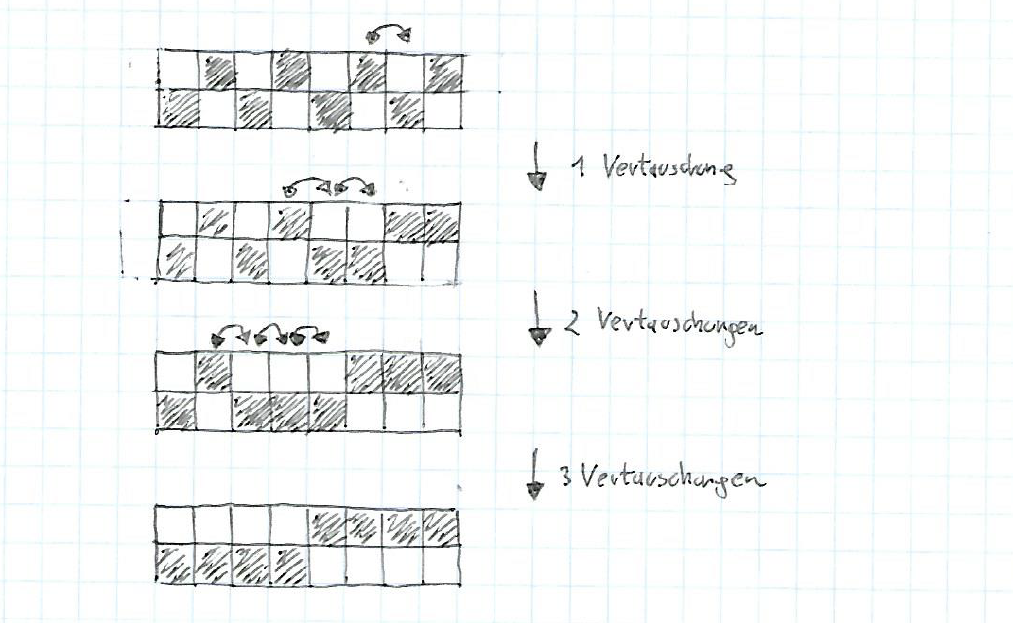
\includegraphics[width = 1\textwidth]{Graphix/Permutation.PNG}
\caption{Veranschaulichung der Permutation $P$ der Zeilen bzw. Spalten von $\bm{M}_I$}
\label{Abb: Permutation für M_I}
\end{figure}
